\begin{center}

\vspace*{1cm}

%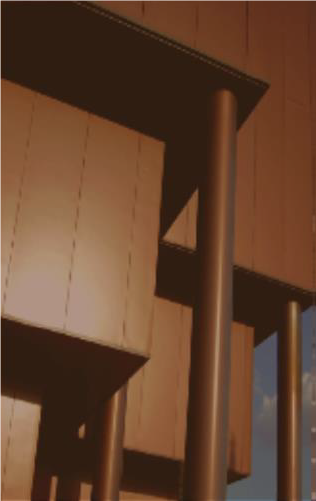
\includegraphics[width=0.25\textwidth]{fig/ilustracion.png}

\includegraphics[width=0.4\textwidth]{fig/miscdg-2.png}

%{\color{US_red} \rule{\linewidth}{0.75mm} }


\vspace*{2cm}
\begin{large}
TRABAJO FIN DE MÁSTER
\end{large}

\vspace*{0.1in}
%Versión en amarillo
\AddToShipoutPictureBG*{\AtPageLowerLeft{%
  \color{US_red!20}\rule{.25\paperwidth}{\paperheight}}}
%versión en rojo
%\AddToShipoutPictureBG*{\AtPageLowerLeft{% \color{US_red!20}\rule{.3\paperwidth}{\paperheight}}}
  
\textbf{\huge Título del trabajo} % Aquí el título de su trabajo

\vspace*{.2in}

{\large Realizado por}\\
\textbf{\Large Sergio Álvarez Piñón} % Aquí su nombre

\vspace*{2cm}
\begin{mdframed}[style=US_style]
\centering
\textbf{Para la obtención del título de}\\
{\large Máster en Ingeniería del Software: Cloud, Datos y Gestión TI} 

\vspace*{0.2in}

\textbf{Dirigido por}\\
{\large José María Luna Romera}\\ % Repetir esta línea si hay más de un tutor

\vspace*{0.2in}
\end{mdframed}


\vspace*{.6in}
\textbf{Convocatoria de Junio, curso 2025/26} % Adaptar al curso en el que presente el trabajo
\vspace*{0.2in}
\end{center}


\thispagestyle{empty} % Impide que se incluya número de página en la portada
\clearpage\setcounter{page}{1} % Comienza a incluir números de página a partir de aquí
\pagenumbering{roman} % En números romanos